\section{Approach}
In this section, we introduce our proposed reference-free summarization evaluation metric which computes the semantic distribution correlation between generated documents with and without a summary and combines the correlation with compression ratio.

\textbf{Semantic Distribution Correlation (SDC).}
Inspired by Shannon score~\cite{shannon22},
we use auto-regressive language model to obtain 
the semantic information of documents.
Given a document $D=\{x_1,x_2,...,x_n\}$ consisting of tokens $x$, 
the auto-regressive language model represents $D$ by
factorizing the joint probabilities over
symbols as the product of conditional probabilities: 
\begin{equation}
	P(D) = \prod_{t=1}^{n}p(x_t|x_{<t})
\end{equation}

In this paper, 
unlike previous metrics using $P(D)$ as the semantic information of $D$, 
we take $p(x_t|x_{<t})$ as the semantic representation of $x_t$
and use a vector $\mathbf{P}(D)$
to represent the semantic distribution of $D$ generated by language model:
\begin{equation}
	\mathbf{P}(D)=\left[p(x_1),p(x_2|x_{<2}),..., p(x_n|x_{<n})\right]
\end{equation}
Such fine-grained semantic representation considers
both the order and semantic of the tokens in sequence,
which helps to evaluate the coherence and relevance.

To evaluate the quality of a summary $S$ consisting of token $y$, we use language model
to predict $D$ with $S$ as a prompt.
The better the summary, the better the document can be restored.
In other words, a better summary makes the semantic information of documents generated with a summary more similar to that of documents generated without summary.
We calculate the semantic distribution of $D$ given $S$ as:
\begin{align}
\mathbf{P}(D|S)=\left[p(x_1|S),p(x_2|x_{<2},S),..., \notag\right.
\\
\left.
p(x_n|x_{<n},S)\right]
\end{align} 
The $P(D)$ and $P(D|S)$ are illustrated in \figref{fig:app}.

\begin{figure}[th]
	\centering
	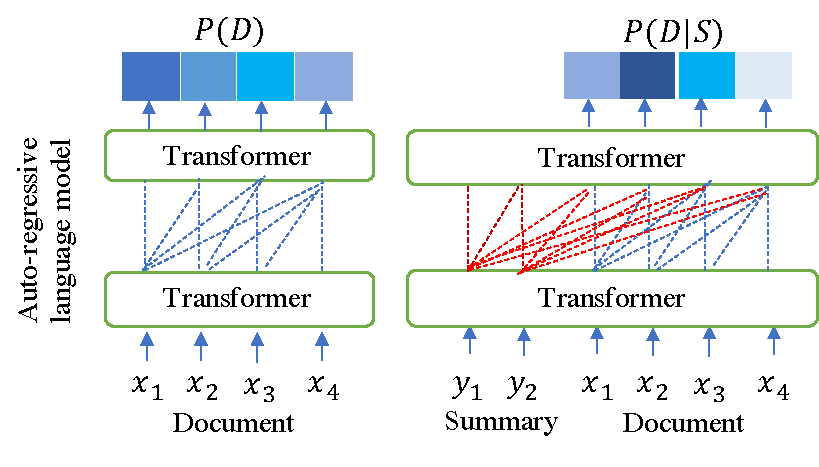
\includegraphics[width=1.0\linewidth]{app.pdf}
	\caption{Architecture of semantic distribution from auto-regressive language model.}
	\label{fig:app}
\end{figure}

We take the correlation between $\mathbf{P}(D)$ and $\mathbf{P}(D|S)$ as the evaluation score of summary $S$:
\begin{align}
	C(D,S)&=Corr(\mathbf{P}(D), \mathbf{P}(D|S)) \\
	W(D,S)&=  \frac{\prod{P(D|S)}}{\prod{P(D)}} \\
	SDC(D,S)&=  W(D,S) \times C_{norm}(D,S)
\end{align}
where $Corr$ is 
Pearson's $\gamma$~\cite{pearson} because we need the change trend of the two distributions for semantic order and need their specific values for information coverage judgement. $W(D,S)$ indicates the extent to which the document $D$ can be predicted by given summary $S$.
Better summaries can get higher $W(D,S)$ scores.
$C_{norm} \in \left[0,1\notag\right)$ is the normalization of $C$.
The higher SDC means the better summary quality.

\textbf{SDC with Compression Ratio (SDC*).}
Compression ratio reflects the difficulty of summarizing,
which is the length of summary divided by the length of source document:
$CR(D, S)=L(S)/L(D)$, where $L$ records the length of text. If $L(S)$ is greater than $L(D)$, $CR(D, S)$ is equal to 1.
It is more difficult to generate a shorter summary.
Thus, we introduce compression ratio into SDC and get SDC* as:
\begin{equation}
	\label{eq:final}
	SDC^*(D, S)=2 \times \frac{SDC\times (1-CR)}{SDC + (1-CR)}
\end{equation}

SDC*  ensures that a summary with higher semantic distribution correlation and lower compression ratio achieves a higher evaluation score.
